The deterministic model is the well known SIRS system, where the population is divided in three compartments: Susceptibles S(t), Infected I(t) and Recovered R(t). \\
 The main assumptions are the following: 
 \begin{enumerate}
    \item recovered patients gain a temporal immunity, reentering the susceptible class at the end of it;
    \item birth and death rate ($\mu$) are equal, thus the total population is constant;
    \item $\nu$ is the recovery rate, while $\gamma$ is the immunization rate;
    \item the transmission coefficient is described by the function $\beta(t)$, which is a continuous T-periodic function, we approximated it by the sinusoidal function $\beta(t) = b_{0}(1 + b_{1}*cos(2\pi*t + \Phi))$\cite{weber}. $b_{0}$ is the baseline transmission rate, $0<b_{1}<1$ measures the amplitude of the seasonal variation in transmission and $0<\Phi<2\pi$ is the phase angle normalized.
\end{enumerate}
 The final model is written as follows:
 \begin{gather}
    \begin{aligned}
    \dot{S}(t) &= \mu - \mu S(t) - \beta (t) S(t) I(t) + \gamma R(t), \ S(0)=S_{0} > 0  \\
    \dot{I}(t) &= \beta (t) S(t) I(t) - \nu I(t) - \mu I(t), \ I(0)=I_{0} > 0  \\
    \dot{R}(t) &= \nu I(t) - \mu R(t) - \gamma R(t), \ R(0)=R_{0} > 0 
    \end{aligned}
 \label{eq:System1}
 \end{gather}
 
 The transmission parameters are missing, so the model is fitted to real hospitalization data of children younger than 4 years old retrieved from Valencia databases, the period span from January 2001 to December 2004.
 The model is fitted through least-squares, using the mean square error function in Mathematica. The error function is minimized through the Nelder-Mead algorithm (Fig. \ref{fig:det_fitting}).

 \begin{figure}[h!]
  \centering
  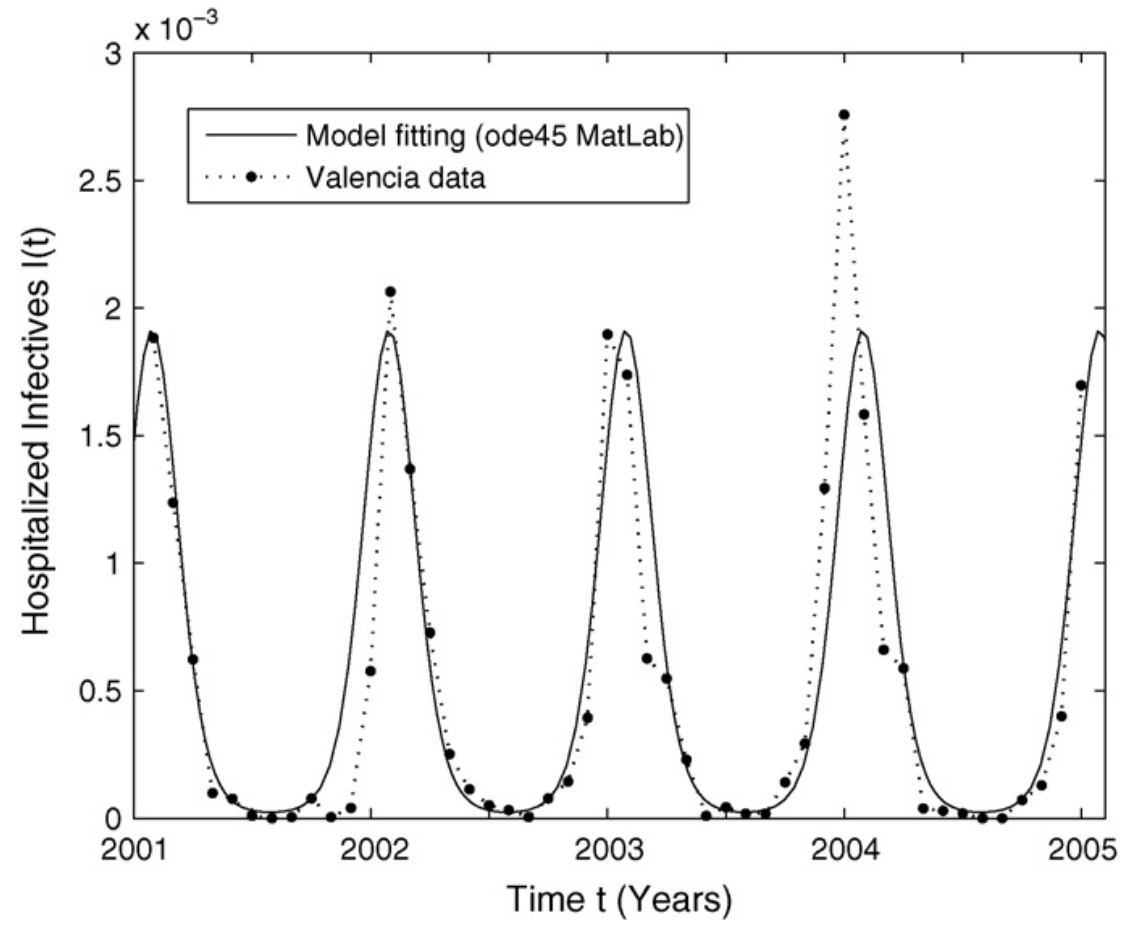
\includegraphics[width=0.8\textwidth]{IMG/det_fitting.png}
  \caption{Parameter estimation of the deterministic model using RSV hospitalization data. The authors point out how the behaviour of the real data is not periodic as in the deterministic model.}
  \label{fig:det_fitting}
\end{figure}

 In the end the function is minimized by the following parameters: \{$b_{0}$, $b_{1}$, $\Phi$, s\} = \{36.4, 0.38, 1.07, 220000\}, where s is the proportion of infected that is not hospitalized.
 The other missing parameters are not directly specified in the paper, consequently we choose them from the literature \cite{weber}, eventually we selected \{$\mu$, $\nu$, $\gamma$\}=\{0.009, 36, 1,8\}. \\
 The initial conditions for S(t), I(t) and R(t) are the same in all simulations, with values 0.9988, 0.0012 and 0 respectively. 